\documentclass[12pt,reqno]{amsart}

\usepackage{graphicx}

\usepackage{amssymb}
\usepackage{amsthm}
\usepackage{mathrsfs}
\setlength{\parskip}{0.5\baselineskip}%
\setlength{\parindent}{20pt}
\theoremstyle{plain}

\newtheorem*{thm*}{Theorem}
%% this allows for theorems which are not automatically numbered

\renewcommand{\qedsymbol}{$\blacksquare$}
\newtheorem{thm}{Theorem}
\newtheorem{lem}{Lemma}
\newtheorem{cor}{Corollary}
\theoremstyle{definition}
\newtheorem{defn}{Definition}
\newtheorem{exer}{Exercise}
\newtheorem{eg}{Example}
\newtheorem{rem}{Remark}
\newtheorem*{sol*}{Solution}
\newcommand{\bb}[1]{\mathbb{#1}}
\newcommand{\cal}[1]{\mathcal{#1}}
\usepackage{lineno}

%% The above lines are for formatting.  In general, you will not want to change these.


\title{General Topology}
\author{Devansh Tripathi}

\begin{document}

\begin{abstract}
    We shall learn some general topology. Rest of the abstract is left as an exercise to the reader.
\end{abstract}
\maketitle
\newpage
\begin{defn}
    Induced metric: A metric which is derived from a norm. A normed space is a special metric space whose metric is derived from a norm.
\end{defn}
\begin{eg}
    $\mathscr{C}[a,b]$: Set of all bounded continuous real function on a closed interval form the normed space with norm defined as $$ \|f\| = \int_a^b |f(x)|~dx \hspace{0.35cm}\text{or,} \hspace{0.5cm} \|f\| = \sup{|f(x)|}$$ and the induced metric is $$ \|f - g \| = \int_a^b |f(x) - g(x)| ~ dx \hspace{0.35cm} \text{or,} \hspace{0.5cm} \|f - g\| = \sup{|f(x) - g(x)|} $$
\end{eg}
\begin{defn}
    Distance of a point $x$ from a set $A$: $$ d(x, A) = \inf\{d(x,a) \mid \forall a \in A \} $$
    Diameter of the set: $$ d(A) = \sup \{d(a_1, a_2) \mid \forall a_1, a_2 \in A\} $$
\end{defn}
\begin{defn}
    Bounded mapping: A mapping $f$ of a non-empty set into a metric space is said to be bounded if its range is bounded i.e. $\exists M \in \mathbb{R} \text{ such that } |f(x)| \leq M $ 
\end{defn}
\begin{eg}
    A pseudo metric which is not a metric
    $$ f,g \in \mathbb{R}^2 \text{ and } d(f,g):= \text{difference between their $x$ coordinates} $$    
\end{eg}
\begin{defn}
    Interval: A set $A \subset \mathbb{R}$ is an interval if $$ \forall x, y \in A \text{ and } \forall t \in \mathbb{R} \colon x \leq t \leq y \implies t \in A $$ 
\end{defn}
\begin{thm}
    Union of intervals with non empty intersection is an interval.    
\end{thm}
\begin{proof}
    Let $\{I_i\}$ be the set of interval and $a \in \cap_i I_i$.\\
    Proof Idea: Take any two points in the union and show that they contains every point in between them (take general point and show that it will belong to the union).\\
    Let $x,y \in \cup_i I_i$ and let $t \in \mathbb{R} \colon x \leq t \leq y $ then there are following possiblities:\\
    $t < a$, \\$ t = a$ or, \\ $t > a$.\\ All are trivial to show that they lie in union.
\end{proof}
\section{Topological Spaces}
\begin{defn}
    Topology: A topology on a set $X$ is a collection $\mathcal T$ of subsets of $X$ having the following properties:
\begin{itemize}
    \item $\phi$ and $X$ are in $\mathcal T$.
    \item The union of the elements of any subcollection of $\mathcal T$ is in $\mathcal T$.
    \item The intersection of the elements of any finite subcollection of $\mathcal T$ is in $\mathcal T$.
\end{itemize}
\end{defn}
A set $X$ with topology $\mathcal T$ is called an topological space ($X,\mathcal T$).
\begin{defn}
    Open set of $X$: For the topological space $(X, \mathcal T)$, a subset $U$ of $X$ is an open set of $X$ if $U$ belongs to the collection $\mathcal T$.
\end{defn}
\begin{eg}
    Discrete Topology: If $X$ is any set then collection of all subsets of $X$ is a topology on $X$, called {\bf discrete topology.}
\end{eg}
\begin{eg}
    Indiscrete or trivial topology: The topology consisting of only $\phi$ and the whole set $X$ is called {\bf trivial topology.}
\end{eg}
\begin{eg}
    Finite complement topology: Let $X$ be a set and $\mathcal{T}$ be the collection of all subset $U$ of $X$ such that $X - U$ is either finite or $X$. Then $\mathcal{T}$ is called {\bf finite complement topology}. (This topology is consists of subset of $X$ whose complement is either finite or $X$.)
\end{eg}
\begin{proof}
    Let $\{U_{i}\}$ be the indexed family of subsets of $X$ belongs to $\mathcal{T}$. $\phi$ and $X$ are obviously there. Assume each $\bigcup\limits_i U_i$ is non-empty (trivial for empty case): 
    $$X - \bigcup\limits_i U_i = \bigcap\limits_i(X - U_i)$$
    Since each $U_i$ is in $\mathcal{T}$, $X - U_i$ is finite. and $\bigcap\liminf_i X - U_i$ is contained in every $X - U_i$ hence it is finite.\\ \\
    To show $\bigcap\limits_i^n X - U_i$ is in $\mathcal{T}$, 
    $$ X - \bigcap\limits_i^n U_i = \bigcup\limits_i^n (X - U_i) $$
    Rhs is finite union of finite sets hence it is finite.
\end{proof}
\begin{eg}
    Let $X$ be set and $\mathcal{T}_c$ be the collection of all subsets $U$ of $X$ such that $U^c$ is either countable or all of $X$. Then $\mathcal{T}_c$ is a topology of $X$. 
\end{eg}
\begin{proof}
    $\phi$ and $X$ are trivial inside $\mathcal{T}_c$. Let $U_i$ be the indexed family of subsets of $X$. Assume $\bigcup\limits_i U_i$ is non-empty (trivial for empty case). To show that $\bigcup\limits_i U_i$ is in $\mathcal{T}_c$
    $$ X - \bigcup\limits_i U_i = \bigcap\limits_i (X - U_i)$$
    Since, $X - U_i$ is countable for each $i$ and $\bigcap\limits_i (X - U_i)$ is in $U_i$ for each $i$. Hence, $\bigcap\limits_i (X - U_i)$ is countable. \\
    To show that $\bigcap\limits_i U_i$ is in $\mathcal{T}_c$, use the same argument as last example and the fact that finite union of countable sets is countable.
\end{proof}
\begin{defn}
    Finer or strictly finer topology: For a set $X$, if $\mathcal{T}$ and $\mathcal{T}'$ are two topologies on $X$ such that $\mathcal{T} \subset \mathcal{T}'$ then we say $\mathcal{T}'$ is {\bf finer} than $\mathcal{T}$ and if $\mathcal{T}'$ properly contains $\mathcal{T}$ then we say it's {\bf strictly finer}. Then $\mathcal{T}$ is called {\bf coarser} than $\mathcal{T}'$ or, {\bf strictly coarser} if it is contained in $\mathcal{T}'$ properly.
\end{defn}
\begin{defn}
    Comparable: We say $\mathcal{T}$ is comparable with $\mathcal{T}'$ if either $\mathcal{T} \subset \mathcal{T}'$ or $\mathcal{T}' \subset \mathcal{T}$.
\end{defn}
\section{Basis for a Topology}
\begin{defn}
    If $X$ is a set, a {\bf basis} for a topology on $X$ is a collection $\mathcal{B}$ of subsets of $X$ (called basis elements) such that
    \begin{itemize}
        \item For each $x \in X$, there is atleast one basis element $B \in \mathcal{B}$ such that $x \in B$.
        \item If $x$ belongs to the intersection of two basis elements $B_1$ and $B_2$, then there is $B_3 \in \mathcal{B}$ such that $x \in B_3 \subset B_1 \cap B_2$. 
    \end{itemize}
\end{defn}
We define a topology $\mathcal{T}$ generated by $\mathcal{B}$ as: A subset $U$ of $X$ is said to be open in $X$ (e.g. an element of topology on $X$) if for all $x \in U$, there is a basis element $B \in \mathcal{B}$ such that $x \in B \subset U$.

\begin{rem}
    Each element of the basis is an element of the topology. 
\end{rem}
\begin{eg}
    If $X$ is any set then the collection of all one element subsets of $X$ is a basis for the discrete topology on $X$.(Power set of $X$). 
\end{eg}
\begin{proof}
    Trivial to see. (Caution: Do not take element of the topology on $X$. For basis, condition is on the elements of the set $X$ hence take element of $X$ and then check basis conditions.)
\end{proof}
\begin{lem}
    The collection $\mathcal{T}$ generated by the basis $\mathcal{B}$ is a topology.
\end{lem}
\begin{proof}
    Let the collection $\mathcal{T} = \{U_i\}_{i \in I}$. Condition for the set $U_i$ to belong to the collection is that for each $x \in U_i$ there exists an element $B \in \mathcal{B}$ and $x \in B \subset U_i$.
    \paragraph{\bf Membership of $\phi$ and $X$:}
    For $\phi$, it is vacuously true (true due to non-availability of elements in the set). For $X$, for each $x \in X$, there exists $B \in \mathcal{B}$ (by definition of basis) such that $x \in B$ and $B \subset X$.
    \paragraph{\bf Closure under arbitray union of elements.} Now, assume that $\{U_i\}_{i \in I}$ is the indexed family of subsets of $X$ which are elements of $\mathcal{T}$. We need to show that $\bigcup\limits_{i \in I} U_i \in \mathcal{T}$. For each $x \in \bigcup\limits_{i} U_i \implies x \in U_i$ for some $i$ and $U_i \in \mathcal{T} \implies \exists B \in \mathcal{B} \text{ such that } x \in B \subset U_i$. This completes the argument.
    \paragraph{\bf Closure under finite intersection.} We need to show that $\bigcap\limits_{i = 0}^{n} U_i \subset \mathcal{T}$. For each $x \in \bigcap\limits_{i = 0}^{n} U_i$
    $$ x \in U_i ~~\forall i \implies \exists B_i \in \mathcal{B} ~~\forall i \in \{0,1,\dots n\}$$
    Since, $x \in \bigcap\limits_{i = 0}^{n} B_i$ and $B_i~'s$ are basis elements hence by definition of basis, $\exists B' \in \mathcal{B}$ such that $x \in B' \subset \bigcap\limits_{i = 0}^{n} B_i$. Hence, $\bigcap\limits_{i = 0}^{n} U_i \subset \mathcal{T}$.
\end{proof}
\begin{lem}
    Let $X$ be a set; $\mathcal{B}$ is the set of all basis elements of the topology $\mathcal{T}$ on set $X$. Then $\mathcal{T}$ equals the collection of all unions of elements of $\mathcal{B}$.
\end{lem}
\begin{proof}
    Since each element $B$ of basis is in $\mathcal{T}$ and hence their union. For other way around, let $U \in \mathcal{T}$, then for each $x \in U~~\exists B_x \in \mathcal{B} \subset U$ hence, $ U = \bigcup\limits_{x \in U} B_x$. Therefore, each $U \in X$ is union of basis elements.
\end{proof}
\begin{rem}
    Above lemma states that every set $U$ in $X$ can be expressed as union of basis elements of the topology, however this is {\bf not unique.}
\end{rem}
\begin{lem}
    Let $X$ be an topological space. Suppose that $\mathcal{C}$ is a collection of open sets of $X$ such that for each open set $U$ of $X$ and each $x \in U$, there is an element $C$ of $\mathcal{C}$ such that $x \in C \subset \mathcal{C}$. Then $\mathcal{C}$ is a basis of the topology of $X$.
\end{lem}
\begin{proof}
    First we will prove that $\mathcal{C}$ is the basis of the topology on $X$.
    \paragraph{\bf First condition of basis:} Since $X$ is a open set of itself hence hypothesis, by for each $x \in X$ there exists $C \in \mathcal{C}$ such that $x \in C \subset \mathcal{C}$.
    \paragraph{\bf Second condition of basis:} Let $x \in C_1 \cap C_2$ for some open sets $C_1, C_2 \in \mathcal{C}$. Since $C_1, C_2$ are open in $X$ then so is $C_1 \cap C_2$ hence by hypothesis for each $x \in C_1 \cap C_2$ there exists $C_3 \in \mathcal{C}$ such that $x \in C_3 \subset C_1 \cap C_2$.
    \paragraph{\bf Topology generated by $\mathcal{C}$ equals topology of $X$.} Let $\mathcal{T}_c$ be the topology generated by $\mathcal{C}$ and $\mathcal{T}$ be a topology on $X$. Let $U \in \mathcal{T}$. For each $x \in U$, by hypothesis, there exists $C_x \in \mathcal{C}$ such that $x \in C_x \subset U$ hence $U = \bigcup\limits_{x \in U} C_x$(union of elements of $\mathcal{C}) \implies \mathcal{T} \subset \mathcal{T}_c$.\\
    Let $V \in \mathcal{T}_c \implies V = \bigcup\limits_{i \in I} C_i$ for each $C_i \in \mathcal{C}$ (by previous lemma). Since each $C_i$ are open in $X$ hence $C_i \in \mathcal{T}$ and $\mathcal{T}$ is a topology (their union will belong to $\mathcal{T}$). Hence, $V \in \mathcal{T} \implies \mathcal{T}_c \subset \mathcal{T}$. Therefore, $\mathcal{T}_c = \mathcal{T}$.
\end{proof}
\begin{lem}
    Let $\mathcal{B}$ and $\mathcal{B}'$ be bases for the topologies $\mathcal{T}$ and $\mathcal{T}'$, respectively, on $X$. TFAE
    \begin{enumerate}
        \item $\mathcal{T}'$ is finer than $\mathcal{T}.$
        \item For each $x \in X$ and each basis element $B \in \mathcal{B}$ containing $x$, there is a basis element $B' \in \mathcal{B}'$ such that $x \in B' \subset B$.
    \end{enumerate}
\end{lem}
\begin{proof}
    $(1) \implies (2)$ (Idea is: Since $\mathcal{T} \subset \mathcal{T}'$, every set of $\mathcal{T}$ is a set in $\mathcal{T}'$. Hence, $B \in \mathcal{T}$ can be written in terms of basis of $\mathcal{T}'$)
    \par \noindent We assume that $\mathcal{T} \subset \mathcal{T}'.$ For all $x \in X$ there exists $B \in \mathcal{B}$ such that $x \in B \subset \mathcal{T}$. And $\mathcal{T} \subset \mathcal{T}' \implies B \subset \mathcal{T}'$. Therefore, there exists a $B' \in \mathcal{B}'$ such that $ \forall x \in B, x \in B' \subset B$.
    \paragraph{$(2) \implies (1)$} Assume $(2)$ and let $U \in \mathcal{T}$. We need to show that $U \in \mathcal{T}'$. For each $x \in U$ there exists $B \in \mathcal{B}$ such that $x \in B \subset U$. From condition $(2)$, there exists a $B' \in \mathcal{B}'$ such that $x \in B' \subset B \subset U \implies B' \subset U$. Therefore by definition of basis, $U \in \mathcal{T}' \implies \mathcal{T} \subset \mathcal{T}'$.
\end{proof}
\begin{defn}[Standard Topology on $\mathbb{R}$]
    If $\mathcal{B}$ is the collection of all open intervals in the real line
    $$ (a,b) = \{x \mid a < x < b\},$$
    the topology generated by $\mathcal{B}$ is called the {\bf standard topology} on the real line.
\end{defn}
\begin{defn}[Lower limit topology on $\mathbb{R}$]
    If $\mathcal{B}'$ is the collection of all half-open interval of the form 
    $$ [a,b) = \{x \mid a \leq x < b\},$$
    where $a < b$, the topology generated by $\mathcal{B}'$ is called the {\bf lower limit topology} on $\mathbb{R}$. $\mathbb{R}$ with this topology is denoted as $\mathbb{R}_l$.
\end{defn}
\begin{defn}[$K$-topology on $\mathbb{R}$]
    Let $K$ denote the set of all number of the form $1/n$, for $\mathbb{Z}_+$, and let $\mathcal{B}$ be the collection of all open intervals $(a,b)$, along with all the set of the form $(a,b) - K$. Then the topology generated by $\mathcal{B}$ is called {\bf $K$-topology} on $ \mathbb{R}$. $\mathbb{R}$ with this topology is denoted as $\mathbb{R}_K$.
\end{defn}
\par The open sets in $K$-topology are of the form $U\backslash C$ where $U$ is open set in standard topology and $C \subset K$.
\begin{exer}
    Prove that the set $\mathcal{B} = \{(a,b) \mid a < b\} \cup \{(a,b) \backslash K \mid a < b\}$ is a basis of the topology on $\mathbb{R}$.
\end{exer}
\begin{sol*}
    First condition of the basis is trivially satisfied since it contains the basis of standard topology.\\
    For second condition: Let $x \in \mathbb{R}$ such that $x \in B_1 \cap B_2$, we need to show that there exists a $B_3 \in \mathcal{B}$ such that $x \in B_3 \subset B_1 \cap B_2$.
    \paragraph{\bf Case 1} If $B_1 = (a,b)$ and $B_2 = (a,b) - K$ then $B_1 \cap B_2 = B_2$ (which can be taken as $B_3$.)
    \paragraph{\bf Case 2} If $B_1 \cap B_2$ are disjoint then $x \notin B_1 \cap B_2$.
    \paragraph{\bf Case 3} If $B_1 = (a,b)$ and $B_2 = (c,d) - K$ with $c \in (a,b)$ and $d > b$ then $B_1 \cap B_2 = (c,b) - K = B_3$.
\end{sol*}
\begin{lem}
    The topologies of $\bb{R}_l$ and $\bb R_K$ are strictly finer than the standard topology on $\bb R$, but are not comparable with one another.
\end{lem}
\begin{proof}
    Let $\mathcal{T}, \cal T', \cal T''$ are the topologies of $\bb R, \bb R_l, \bb R_K$. We want to show $\cal T \subsetneq \cal T'$ and $\cal T \subsetneq \cal T''$. For each $x \in \bb R$ and given a basis element $(a,b) \in \cal B_{\bb R}$ containing $x$, there exists $[x,b) \in \cal B_{\bb R_l}$ and $(a,b) \in \cal B_{\bb R_K}$ such that $x \in [x,b) \subset (a,b)$ and $x \in (a,b) \subset (a,b)$. By previous lemma $\cal T \subset \cal T'$ and $\cal T \subset \cal T''$.
    \par Now, for each $x \in \bb R$ and given $[x,b) \in \cal B_{\bb R_l}$ and $(-1,1) - K \in \cal B_{\bb R_K}$ there does not exists an open interval $(a,c)$ where $c < b$ in $\cal T$ containing $x$ but contained in $[x,b)$ and there does not exists an open interval $(c,d) \in \cal T$ where $c > a$ and $d < b$ containing $0$ such that $x \in (c,d) \subset (a,b) - K$ ($(c,d)$ will contain elements of $K$ but later does not). Hence, $\cal T \subsetneq \cal T'$ and $\cal T \subsetneq \cal T''$. 
    \par For each $x \in \bb R_l$ and given a basis element $[x, b) \in \cal B_{\bb R_l}$ there does not exists $(a,b) - U$ in $\cal T'' $ where $U \subset K$ (it can be $\phi$ for $(a,b)$) such that $x \in (a,b) - U \subset [x,b)$. Also for each $x \in \bb R_K$ and given $(a,b) - U$, where $U \subset K$, containing $x$ there does not exists $[x,b)$ in $\cal T'$ such that $x \in [x,b) \subset (a,b)- U$. Hence $\cal T'$ and $\cal T''$ are not comparable.
\end{proof}
\subsection{Subbasis of a topology}
\begin{defn}[Subbasis]
    A subbasis $\cal{S}$ for a topology on $X$ is a collection of subsets of $X$ whose union equals $X$. The {\bf topology generated by the subbasis $\cal S$} is defined to be the collection $\cal T$ of all unions of finite intersection of elements of $\cal S$. 
\end{defn}
\begin{thm}
    The collection $\cal T$ of all unions of finite intersections of elements of $\cal S$ is a topology.
\end{thm}
\begin{proof} (Idea: We will prove that set of finite intersections of elements of $\cal S$ is a basis then by lemma $2$, $\cal T$ is topology.)
    Let $\cal B$ be the set of finite intersections of elements of $\cal S$. For each $x \in X$, $x \in S_i \in \cal S$ for some $i$ implies there exists $B \in \cal B$ such that $x \in B$. That is first condition for basis. 
    \par Let $x \in B_i \cap B_j$ for some $B_i,B_j \in \cal B$. Since $\cal B$ is a collection of all finite intersections hence there exists $B \in \cal B$ such that $B = B_i \cap B_j$ (intersection of two finite sets is finite.) Therefore, $x \in B \subset B_i \cap B_j$.
\end{proof}
\begin{exer}
    Is the collection $$ \cal T_{\infty} = \{U \mid X - U \text{ is infinite or empty or all of } X\}$$ a topology on $X$?
\end{exer}
\begin{sol*}
    No. For example take $\bb R$. Notice that $\{x\} \in \cal T_{\infty}$. Now, take $\bb R - \cup_{x \neq 0}\{x\}$ is $\{0\}$ which is not infinite. Hence arbitrary union of members of the collection is not in the topology.
\end{sol*}
\begin{rem}
    $\{\cal T_{\alpha}\}$ is the family of topologies on the set $X$ then $\cap \cal T_{\alpha}$ is the topology on the set $X$ while $\cup \cal T_{\alpha}$ may not be the topology on $X$ (union axiom fails). 
    \par $\cup \cal T_{\alpha}$ is the topology on $X$ if they are contained into one another.
\end{rem}
\begin{exer}
    Let $\{\cal T_{\alpha}\}$ be a family of topologies on $X$. Show that there is a unique smallest topology on $X$ containing all the collections $\cal T_{\alpha}$, and a unique largest topology contained in all $\cal T_\alpha$.
\end{exer}
\begin{sol*}
    Since $\cap\{\cal T_\alpha\}$ is the largest collection of sets contained in all $\cal T_\alpha \in \{\cal T_\alpha\}$ and it is a topology (basic application of axioms of topology). For {\bf uniqueness}, let $\cal T'$ be another largest topology contained in all $\cal T_\alpha$ then for some $U \in \cal T'$ implies $U \in \cal T_\alpha$ for all $\cal T_\alpha \in \{\cal T_\alpha\}$ which implies $U \in \cap \{\cal T_\alpha\}$. $\cal T' \subset \cap \{\cal T_\alpha\}$. Other inclusion can also be shown in the similar way. If $U \in \cap\{\cal T_\alpha\}$ then it should be in $\cal T'$ otherwise $\cal T'$ can not be largest. Hence, $\cap\{\cal T_\alpha\} \subset \cal T'$. $\cal T' = \cap\{\cal T_\alpha\}$.

    Let $\{\cal T_i\}$ be the indexed family of topologies such that for all $i \in I$, $\cal T_i$ contains $\{\cal T_\alpha\}$. Then $\cap \{\cal T_i\}$ will be the smallest topology containing $\{\cal T_\alpha\}$. For {\bf uniqueness}, let $\cal T'$ be another such smallest topology then $\cap \{\cal T_\alpha\} \subset \cal T'$ since former is smallest and $\cap \{\cal T_\alpha\} \subset \cal T'$ by taking later as smallest. $\cap \{\cal T_\alpha\} = \cal T'$.
\end{sol*}
\begin{exer}
    Show that if $\cal A$ is a basis for a topology on $X$, then the topology generated by $\cal A$ equals the intersection of all topologies on $X$ that contains $\cal A$. Prove the same if $\cal A$ is a subbasis.
\end{exer}
\begin{sol*}
    To show $\cal T = \cap \{\cal T_i\}$ in the following cases:
    \paragraph{\bf When $\cal A$ is a basis} Let $\cal T$ be the topology on $X$ generated by $\cal A$ implies $\cal T = \cup \cal A$. And assume the family of {\it all} the topologies on $X$, each of one contains $\cal A$, to be $\{\cal T_i\}$. 
    \paragraph{$(\impliedby)$} Since $\cal T \in \{\cal T_i\}$ because $\cal T$ is also a topology on $X$. Hence $\cap \{\cal T_i\}$ is a topology contains in every $\cal T_i$ particularly, $\cap\{\cal T_i\} \subset \cal T$.
    \paragraph{$(\implies)$} Let $U \in \cal T$ implies that $U = \cup \cal A$. Since $\cal A \subset \cal T_i$ for all $i$ and each $\cal T_i$ is a topology hence $\cup \cal A \subset \cal T_i$ for all $i$. Since the union is arbitrary hence $U \subset \cal T_i$ for all $i$ implies $U \subset \cap \{\cal T_i\}$. $\cal T \subset \cap \{\cal T_i\}$. Therefore, $\cal T = \cap \{\cal T_i\}$.
    \paragraph{\bf When $\cal A$ is a subbasis} Let $\cal B$ is the collection of all finite intersections of the elements of $\cal A$. Assume the topology generated by subbasis to be $\cal T = \cup \cal B$ and $\{\cal T_i\}$ to be {\it all} topologies on $X$ each containing $\cal A$.

    \paragraph{$(\impliedby)$} This is same as above case.

    \paragraph{($\implies$)} Let $\cal T = \cup \cal B$. Since each element $B$ of $\cal B$ is finite intersection of elements of $\cal A$, each $B \subset A_i$ for $A_i$'s whose intersection is equal to $B \implies \cal B \subset \cal A$. $\cal A$ is contained in each $\cal T_i \in \{\cal T_i\}$ implies that $\cal B \subset \cap \{\cal T_i\} \implies \cup \cal B \subset \cap \{\cal T_i\}$. This means $\cal T \subset \cap \{\cal T_i\}$.
    \par Therefore, $\cal T = \cap \{\cal T_i\}$.
\end{sol*}
\section{The Order Topology}
\begin{defn}[Order Topology]
    Let $X$ be a set with a simple order relation; assume $X$ has more than one element. Let $\cal B$ be the collection of all the sets of the following types:
    \begin{enumerate}
        \item All open interval $(a,b)$ in $X$.
        \item All intervals of the form $[a_0, b)$ where $a_0$ is the smallest element (if any) of $X$.
        \item All intervals of the form $(a, b_0]$ where $b_0$ is the largest element (if any) of $X$.
    \end{enumerate}
    The collection $\cal B$ is the basis for a topology on $X$ which is called {\bf order topology}.
\end{defn}
Let's check if the set $\cal B$ satisfies the conditions for the basis: for any $x \in X$, there always exists atleast an element of $(1)$ containing it. The smallest element (if any) lies in type $(2)$ and similarly the largest element (if any) lies in type $(3)$. For second condition of the basis: there are several cases that needed to be checked such as $x$ lies in intersection of type $(1)$ and $(1)$, type $(1)$ and $(2)$, type $(1)$ and $(3)$, type $(2)$ and $(3)$ and so on. It can be showed that it satisfies the second condition.

\begin{eg}[Order topology on $\bb Z_+$ is discrete topology]
    $\bb Z_+$ forms ordered set with smallest element. The order topology on $\bb Z_+$ is the discrete topology (Power set topology) because the basis of the discrete topology can be written in the above form. Basis for discrete topology is the set of singleton positive integers. 
    
    \noindent For every one-point set is open: for $n > 1$, the one-point set $\{n\} = (n-1, n+1)$ which is the basis element; and if $n=1$, the one-point set $\{n\} = [1,2)$ which is the element of the basis set.
\end{eg}
\begin{eg}
    The set $X = \{1,2\} \times \bb Z_+$ in the dictionary order is the ordered set with smallest element. The order topology on this set is {\it not } discrete topology. Proof: Let $a_n = 1 \times n$ and $b_n = 2 \times n$ then the element can be ordered as: 
    $$ a_1, a_2, \dots ;b_1, b_2, \dots$$
    Here $a_1$ is the smallest element and $ \{a_1\} = [a_1, a_2)$ which is a basis element. And other elements except $b_1$ can be written as $\{a_n\} = (a_{n-1}, a_{n+1})$ and same for $b_n, n \neq 1$. For $b_1$, it cannot be written as some element of the basis without containing the elements of sequence $a_i$.    
\end{eg}
\begin{defn}[Rays]
    If $X$ is an ordered set, and $a$ is an element of $X$, there are four subsets of $X$ that are called the {\bf rays} determined by $a$. They are the following:
    \begin{enumerate}
        \item $(a, +\infty) = \{x \mid x > a\}$
        \item $(-\infty, a) = \{x \mid x < a\}$
        \item $[a, +\infty) = \{x \mid x \geq a\}$
        \item $(-\infty, a] = \{x \mid x \leq a\}$
    \end{enumerate}
    Sets of first two types are called {\bf open rays} and the last two types are called {\bf closed rays}.
\end{defn}
Open rays are open in order topology as it can be shown as: if there exists an largest element $b_0$ in $X$ then $(a, \infty)$ can be written as $(a,b_0]$ which is the basis element of order topology. (A set is open if it can be written as union of basis elements).

If there does not exists a largest then $(a, \infty)$ can be written as union of $(a, x)$ for $x > a$. In either case $(a,\infty)$ is open. A similar argument applies for $(-\infty, b)$.

\begin{thm}
    The open rays form a subbasis for the order topology $(\cal T)$ on $X$.
\end{thm}
\begin{proof}
    Let the collection of open rays to be $\cal S$. We need to show that $\cal T = \cup (\cap_{i= 1}^{k}\cal S)$ for all $k = 0, 1, \dots$ and for $\cal S$ to be a subbasis.

    \noindent $(\impliedby)$ As we have seen above that open rays are open in order topology and so their finite intersections. Hence, $\cup (\cap_{i= 1}^{k}\cal S) \subset \cal T$ because $\cal T$ is a topology.

    \noindent $(\implies)$ Every basis element of the order topology is the finite intersection of elements of $\cal S$. To see this, $(a,b)$ is intersection of $(a, \infty)$ and $(-\infty, b)$. And if there exists largest $(a_0)$ and smallest $(b_0)$ elements then $[a_0, b)$ and $(a,b_0]$ are themselves open rays. Hence basis of order topology is contained in the set of open rays and this implies $\cal T \subset \cup (\cap_{i= 1}^{k}\cal S)$.
\end{proof}
\section{The Product Topology}
\begin{defn}[Product topology]
    Let $X$ and $Y$ be topological spaces. The {\bf product topology} on $X \times Y$ is the topology having as basis the collection $\cal B$ of all sets of the form $U \times V$, where $U$ is an open subset of $X$ and $V$ is an open subset of $Y$. 
\end{defn}

The collection $\cal B$ forms the basis for product topology. For all $x \times y \in X \times Y$ is contained in the open set $X \times Y$ since $X \times Y$ belongs to $\cal B$. Also intersection of two open sets is open hence their intersection is the element of $\cal B$. Hence second condition of the basis is also satisfied.

\begin{rem}
    The collection $\cal B$ is not the topology on $X$ although it is collection of open sets. To see this, $(U_1 \times V_1) \cup (U_2 \times V_2)$ is open in $X \times Y$ when all individual sets are open but it is not contained in $\cal B$ since it cannot be written as product of two open sets. See figure $\ref{fig:1}$.
    \begin{figure}[!ht]
        \centering{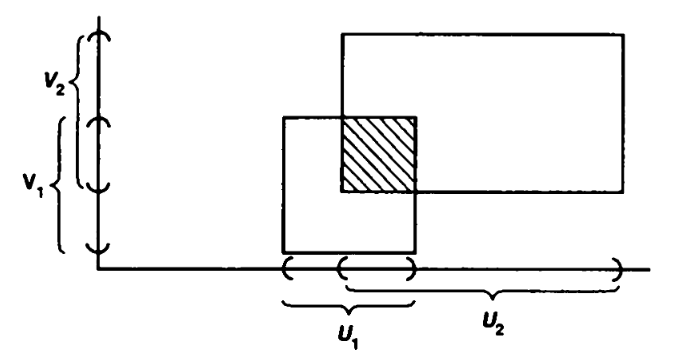
\includegraphics[scale=0.45]{../assests/product_topo.png}}
        \caption{}
        \label{fig:1}
    \end{figure}
\end{rem}

\begin{thm}
    If $\cal B$ is a basis for the topology of $X$ and $\cal C$ is the basis for the topology on $Y$, then the collection
    $$ \cal D = \{B \times C \mid B \in \cal B \text{ and } C \in \cal C\} $$ 
    is a basis for the topology of $X \times Y$.
\end{thm}
\begin{proof}
    Let $W$ be the open subset of $X \times Y$ which is the product topology hence by definition there exist $U \times V \in X \times Y$ such that $U$ is open in $X$ and $V$ is open in $Y$. Since $\cal B$ and $\cal C$ are the bases for topology on $X$ and $Y$ respectively there exists $B \in \cal B$ and $C \in \cal C$ such that for each $x \in U \implies x \in B \subset U$ and for each $y \in V \implies y \in C \subset V$. Therefore, $x \times y \in B \times C \subset U \times V$. Hence by lemma $3$, $\cal D$ is the basis for topology on $X \times Y$.    
\end{proof}

\begin{exer}
        
\end{exer}

\begin{defn}[Projections]
    Let $\pi_1 : X \times Y \to Y$ be defined by the equation
    $$ \pi_1(x,y) = x;$$ 
    let $\pi_2 : X \times Y \to Y$ be defined by the equation
    $$ \pi_2(x,y) = y.$$
    The maps $\pi_1$ and $\pi_2$ are called the {\bf projections} of $X \times Y$ onto $X$ and $Y$ respectively.
\end{defn}
\begin{rem}
    The maps $\pi_1$ and $\pi_2$ are surjective.
\end{rem}
If $U$ is an open set of $X$ then $\pi_1^{-1}(U) = U \times Y$ which is open is $X \times Y$. Similarly, $\pi_2^{-1}(V) = X \times V$ which is open in $X \times Y$.

\begin{thm}
    The collection
    $$ \cal S = \{\pi_1^{-1}(U) \mid U \text{ open in } X\} \cup \{\pi_2^{-1}(V) \mid V \text{ open in } Y\}$$
    is a subbasis for the product topology on $X \times Y$.
\end{thm}
\begin{proof}
    Let $S_{ij} = \pi_1^{-1}(U_i) \cup \pi_2^{-1}(V_j)$. To show that $\cal S$ is subbasis we need to show that $\cup_j(\cup_i S_{ij}) = X$. 
    
    \noindent $(\implies)$ Let $x \in S_{ij}$ implies that $x \in U_i \times Y$ or $x \in X \in V_j$. In either case, $x \in X \times Y$ since $U_i \subset X$ and $V_j \subset Y$. $\cup_j(\cup_i S_{ij}) \subset X \times Y$.

    \noindent $(\impliedby)$ Let $x \in X \times Y$. This case is trivial since $U_i = X$ and $V_j = Y$ and then $x \in (X \times Y) \cup (X \times Y)$. This implies that $x \in \cup_j(\cup_i S_{ij})$. Therefore, $\cup_j(\cup_i)S_{ij} = X \times Y$. 

    TODO
\end{proof}

\begin{defn}[Open map]
    A map $f : X \to Y$ is said to be an {\bf open map} if for every open set $U$ of $X$, the set $f(U)$ is open in $Y$.
\end{defn}

\begin{thm}
    The projection maps $\pi_1 : X \times Y \to X$ and $\pi_2 : X \times Y \to Y$ are open maps.
\end{thm}
\begin{proof}
    Let $U \times V$ be the open set in $X \times Y$ where $U$ is open is $X$ and $V$ is open in $Y$. Since, $\pi_1(U \times V) = U \subset X$ and $U$ is open in $X$. Same argument can be applied for $\pi_2(U \times V)$. This shows that $\pi_1$ and $\pi_2$ are open maps.
\end{proof}

\section{The Subspace topology}
\begin{defn}
    Let $X$ be a topological space with topology $\cal T$. If $Y$ is a subset of $X$, the collection
    $$ \cal T_y = \{Y \cap U \mid U \in \cal T\} $$
    is a topology on $Y$, called the {\bf subspace topology}. With this topology, $Y$ is called the {\bf subspace} of $X$.
\end{defn}
It is easy to check that $\cal T$ is the topology with the fact that 
$$ \bigcup_{i \in I} U_i \cap Y = (\cup_{i \in I} U_i) \cap Y$$

\begin{lem}
    If $\cal B$ is a basis for the topology on $X$ then the collection 
    $$ \cal B_y = \{ B \cap Y \mid B \in \cal B\}$$
    is the basis for the subspace topology on $Y$.    
\end{lem}
\begin{proof}
    Given an open set $U \subset X$. For each $y \in U \cap Y$, since $U \cap Y \subset U$, there exists $B \in \cal B$ such that $y \in B \subset U \cap Y$. Also, $y \in Y$ hence
    $$
    \begin{array}{l}
        y \in B \cap Y \subset B \subset U \cap Y \\
        y \in B \cap Y \subset U \cap Y        
    \end{array} 
    $$
    By lemma $3$, the collection $\{B \cap Y \mid B \in \cal B\}$ is the basis for the subspace topology on $Y$.
\end{proof}
\begin{lem}
    Let $Y$ be a subspace of $X$. If $U$ is open in $Y$ and $Y$ is open in $X$, then $U$ is open in $X$.
\end{lem}
\begin{proof}
    Since $U \in Y$. We have 
    $$
    \begin{array}{l}
        U = \bigcup (U_x \cap Y) \\
        U = (\bigcup U_x) \cap Y \\        
    \end{array}
    $$
    Since, $U_x$'s are open in $X$ so do their arbitrary union and $Y$ is open in $X$. Finite intersection of open sets is open. Hence $U$ is open in $X$.
\end{proof}

\begin{thm}[Relationship between subspace and product topology]
    If $A$ is a subspace of $X$ and $B$ is a subspace of $Y$, then the product topology on $A \times B$ is the same as the topology $A \times B$ inherits as a subspace of $X \times Y$.
\end{thm}
\begin{proof}
    Let $\cal B$ be the basis of the product topology on $A \times B$. 
    $$ \cal B = \{U \times V \mid U \text{ in basis of } A; V \text{ in basis of } B\} $$
    and $\cal B'$ be the basis of the topology $A \times B$ inherits as a subspace of $X \times Y$.
    $$ \cal B' = \{(A \times B)\cap (U_x \times V_y) \mid U_x \times V_y \text{ in basis of } X \times Y\} $$
    We need to show that $\cal B = \cal B'$. 
    
    \noindent $(\implies)$ Since, $A$ is a subspace of $X$ and $B$ is a subspace of $Y$, implies $U = A \cap U_x$ where $U_x$ is in the basis of $X$ and $V = B \cap V_y$ where $V_y$ is in the basis of $Y$. Hence. 
    \begin{align*}
        U \times V &= (A \cap U_x) \times (B \cap V_y)\\
        U \times V &= (A \times B) \cap (U_x \times V_y)        
    \end{align*}
    Last equation can be seen by drawing the figure. Hence, $\cal B \subset \cal B'$.

    \noindent $(\impliedby)$ For any element $(A \times B) \cap (U_x \cap V_y)$ in $\cal B'$, it can be written as $(A \cap U_x) \times (B \cap V_y)$ (can be seen from visualization). Since $U_x$ is in the basis of $X$, $A \cap U_x$ is in the basis of $A$ as a subspace of $X$. Same argument can be extended for $B \cap V_y$.
    \begin{align*}
        (A \times B) \cap (U_x \cap V_y) &= U' \times V'\\
        (A \times B) \cap (U_x \cap V_y) &\in \cal B\\
        \cal B' &\subset \cal B
    \end{align*}
    where $U'$ and $V'$ are  some basis element of $A$ and $B$ respectively. Since, $\cal B = \cal B'$ hence the topology generated by them are equal.
\end{proof}

\begin{rem}
    Let $X$ be an ordered set in the order topology, and let $Y$ be a subset of $X$. Then order relation on $X$, when restricted to $Y$, makes $Y$ into an ordered set.    
\end{rem}
\begin{rem}
    However, the resulting order topology on $Y$ need not be the same as the topology that $Y$ inherits as a subspace of $X$.
\end{rem}

\begin{defn}[Convex set]
    Given an ordered set $X$, A subset $Y$ of $X$ is {\bf convex} in $X$ if for each pair of points $a < b$ of $Y$, the entire interval $(a,b)$ of $X$ is contained in $Y$. 
\end{defn}
\begin{rem}
    The interval and rays in $X$ are convex in $X$.    
\end{rem}
\begin{thm}
    Let $X$ be an ordered set in the order topology; let $Y$ be a subset of $X$ that is convex in $X$. Then the order topology on $Y$ is the same as topology $Y$ inherits as a subspace of $X$.
\end{thm}
\begin{proof}
    
\end{proof}


\end{document}